\documentclass[pdf]{beamer}
\mode<presentation>{}

\usepackage[absolute, overlay]{textpos}
\usepackage[style=verbose-ibid,backend=bibtex]{biblatex}
\bibliography{references}

\title{Layer-skipping connections facilitate training of layered networks using equilibrium propagation.}
\author{Jimmy Gammell \and Sae Woo Nam \and Adam N. McCaughan}
\date{July 28, 2020}

\begin{document}

\section{Title} % Total slide count: 7-12 slides
\begin{frame} % title slide
	\titlepage
\end{frame}

\section{Motivation} % 1-2 slides
\begin{frame}
	\begin{itemize}
		\item<1-> Equilibrium propagation\autocite{scellier17}: biologically-motivated learning framework
		\begin{itemize}
			\item<2-> Simple neurons relative to backpropagation
			\item<3-> Potential application of neuromorphic analog hardware
		\end{itemize}
	\end{itemize}

\end{frame}

\section{Introduction} % 1-2 slides

\section{Procedure} % 1-2 slides

\section{Results} % 3-4 slides

\section{Conclusions} % 1-2 slides



\section{Introduction}
\begin{frame}
	\frametitle{Introduction}
	\begin{itemize}
		\item<1-> Equilibrium propagation is a biologically-motivated learning framework
		\item<2-> Appealing as potential application for neuromorphic analog hardware
		\item<3-> Vanishing gradient problem with conventional layered network topology
		\item<4-> We will show that adding layer-skipping connections can help solve the problem
		\begin{itemize}
			\item<5-> Still biologically-plausible
			\item<6-> Simple to implement in hardware with configurable connectivity
		\end{itemize}
	\end{itemize}
\end{frame}

\section{Background}
\subsection{Equilibrium propagation}
\begin{frame}
	\frametitle{Background: equilibrium propagation}
	\begin{itemize}
		\item<1-> Seminal paper: Equilibrium Propagation: Bridging the Gap Between Energy-Based Models and Backpropagation by Benjamin Scellier and Yoshua Bengio
		\item<2-> Biologically-motivated learning framework
		\begin{itemize}
			\item<3-> For energy-based networks, e.g. continuous Hopfield network
			\item<4-> Gradient descent on cost function
		\end{itemize}
		\item<5-> More biologically-plausible than backpropagation
		\begin{itemize}
			\item<6-> Neurons only need to communicate activation values, not error-correction information
			\item<7-> Prediction (free) and correction (weakly-clamped) phases use same type of computation
		\end{itemize}
		\item<8-> For same reasons, appealing for implementation on neuromorphic analog hardware
	\end{itemize}
\end{frame}

\subsection{Vanishing gradient problem}
\begin{frame}
	\frametitle{Background: vanishing gradient problem}
	\begin{itemize}
		\item<1-> Vanishing gradient problem in conventional layered networks
		\begin{itemize}
			\item<2-> Leads to slow training
			\item<3-> Potential issues in systems with limited bit depth
		\end{itemize}
		\item<4-> Original paper solved by manually tuning an independent learning rate for each layer - unappealing solution
		\begin{itemize}
			\item<5-> More hyperparameters to tune
			\item<6-> Inconvenient to implement in neuromorphic analog hardware
			\item<7-> Seems unlikely to happen in biological systems
		\end{itemize}
	\end{itemize}
\end{frame}

\section{Solution}
\subsection{Description}
\begin{frame}
	\frametitle{Our solution: layer-skipping connections}
	\begin{itemize}
		\item<1-> Our solution: modify layered topology by adding random layer-skipping connections
		\begin{itemize}
			\item<2-> Inspired by small-world topology, but little correlation with common small-worldness metrics (e.g. characteristic path length, clustering coefficient, small-world coefficient)
			\item<3-> Could be conveniently implemented in neuromorphic systems with configurable connectivity
		\end{itemize}
	\end{itemize}
\end{frame}

\subsection{Original topology illustration}
\begin{frame}
	\frametitle{Conventional layered topology}
	\begin{figure}
		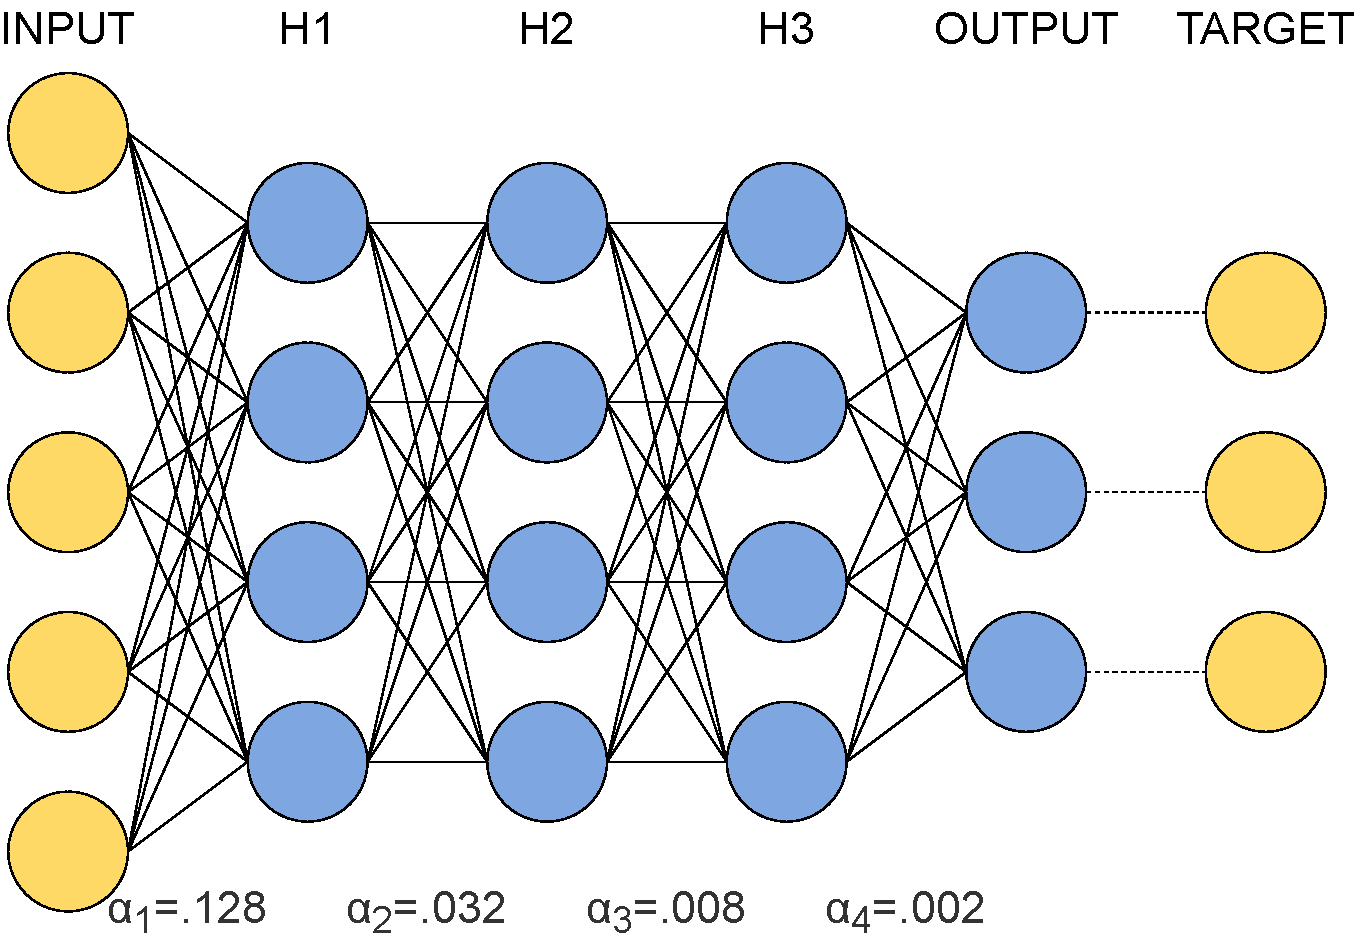
\includegraphics[width=.8\textwidth]{figures/basic_topology_illustration.pdf}
	\end{figure}
	\begin{itemize}
		\item Topology used in original paper
		\item Independently-tuned learning rates for each layer
	\end{itemize}
\end{frame}

\begin{frame} 
	\frametitle{Our topological modifications}
	\begin{textblock*}{.8\textwidth}[.5, .5](.5\paperwidth,.425\paperheight)
		\begin{center}
		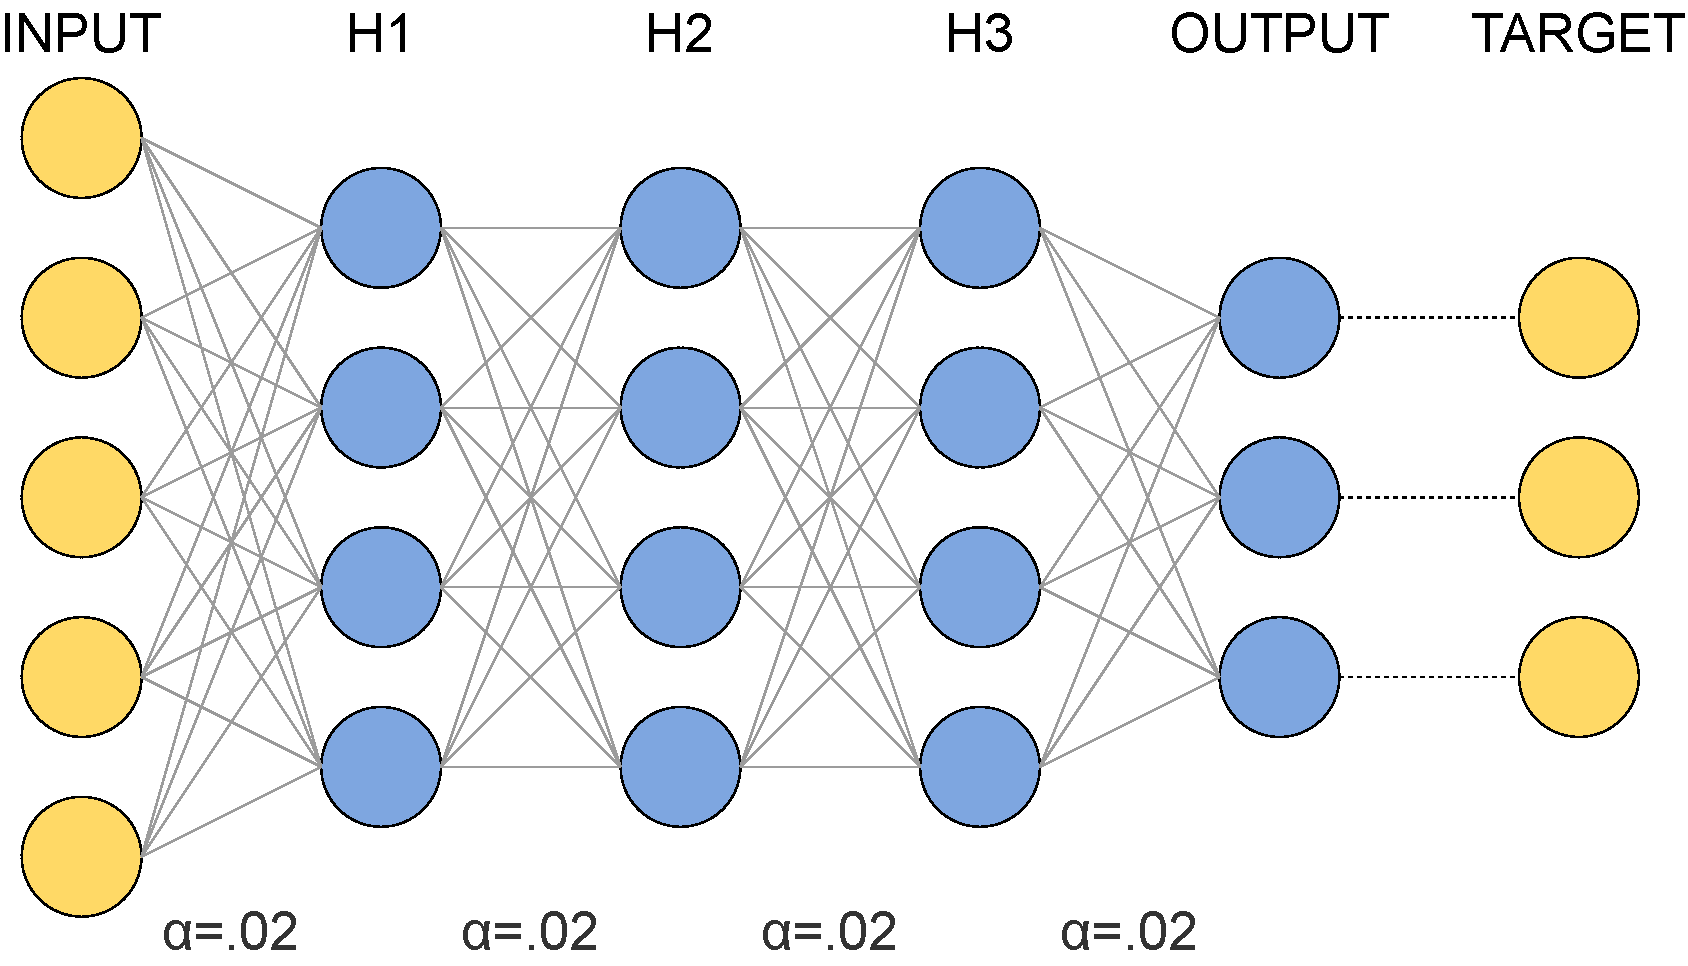
\includegraphics[width=\textwidth]{figures/topology_changes_step1.pdf}<1>
		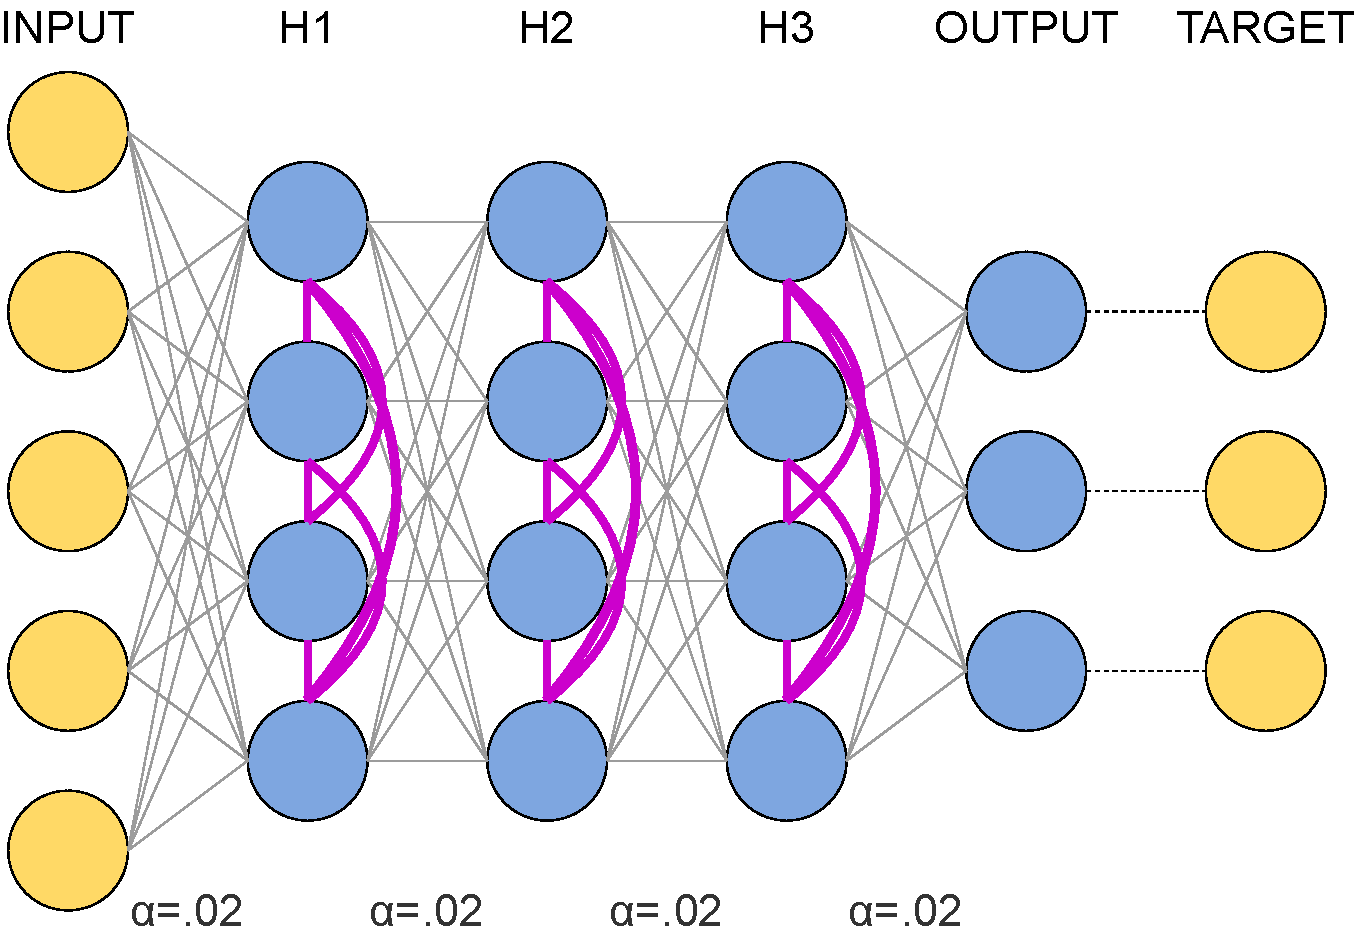
\includegraphics[width=\textwidth]{figures/topology_changes_step2.pdf}<2>
		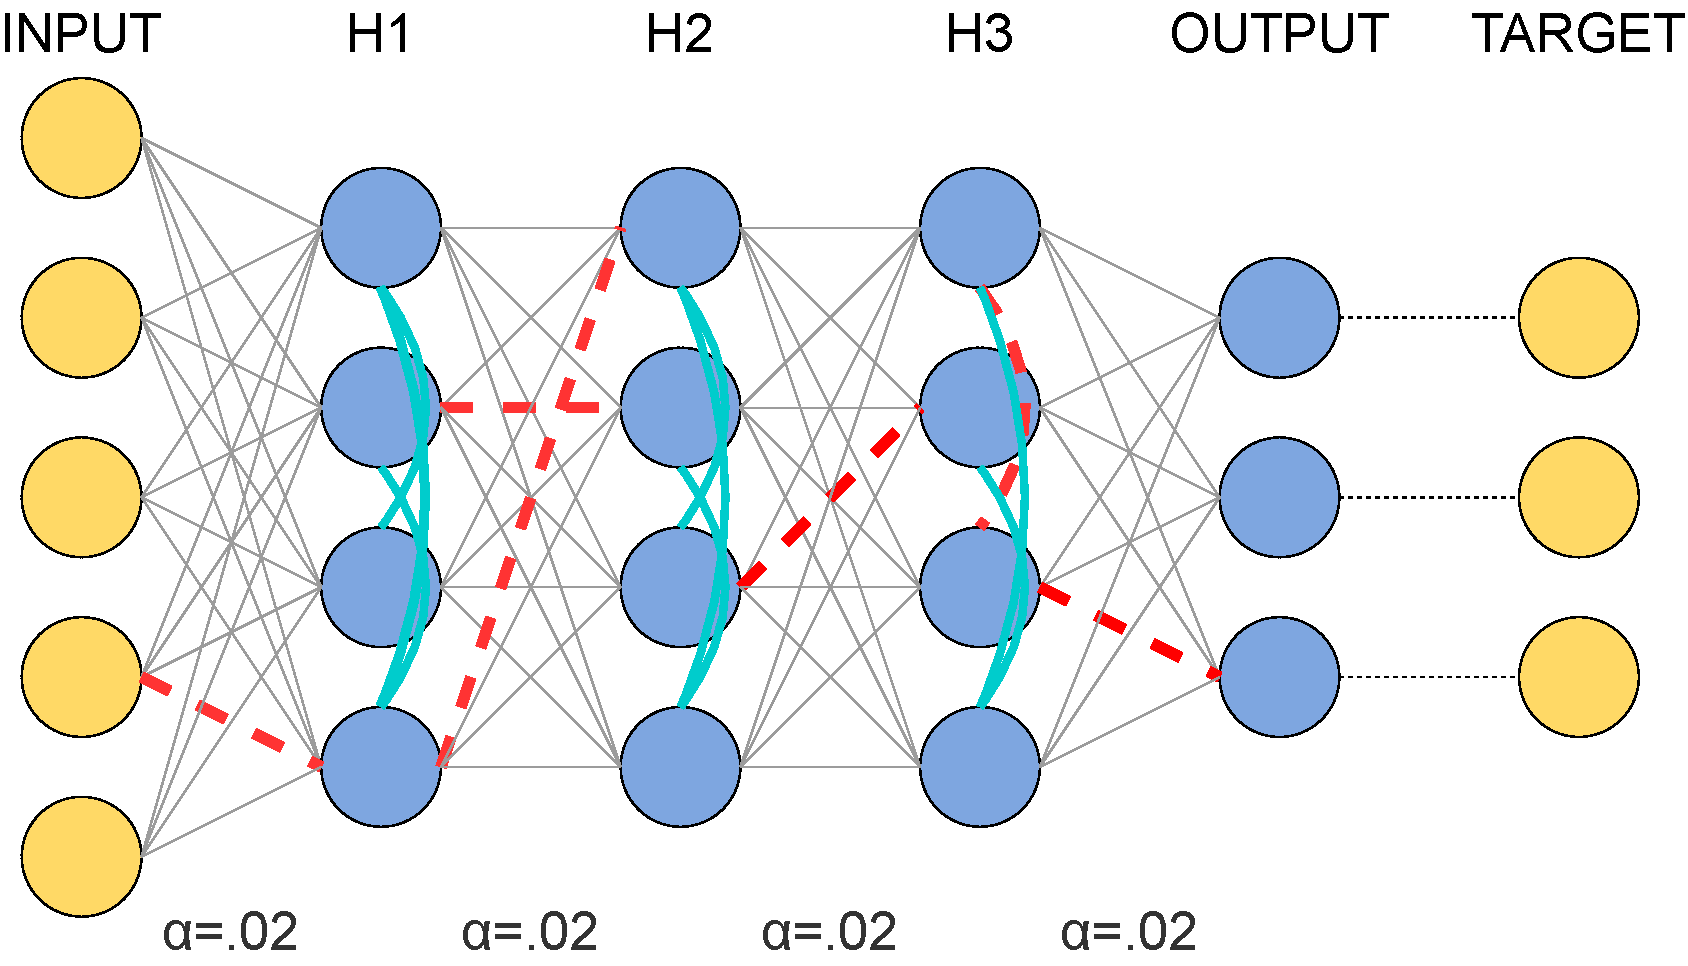
\includegraphics[width=\textwidth]{figures/topology_changes_step3.pdf}<3>
		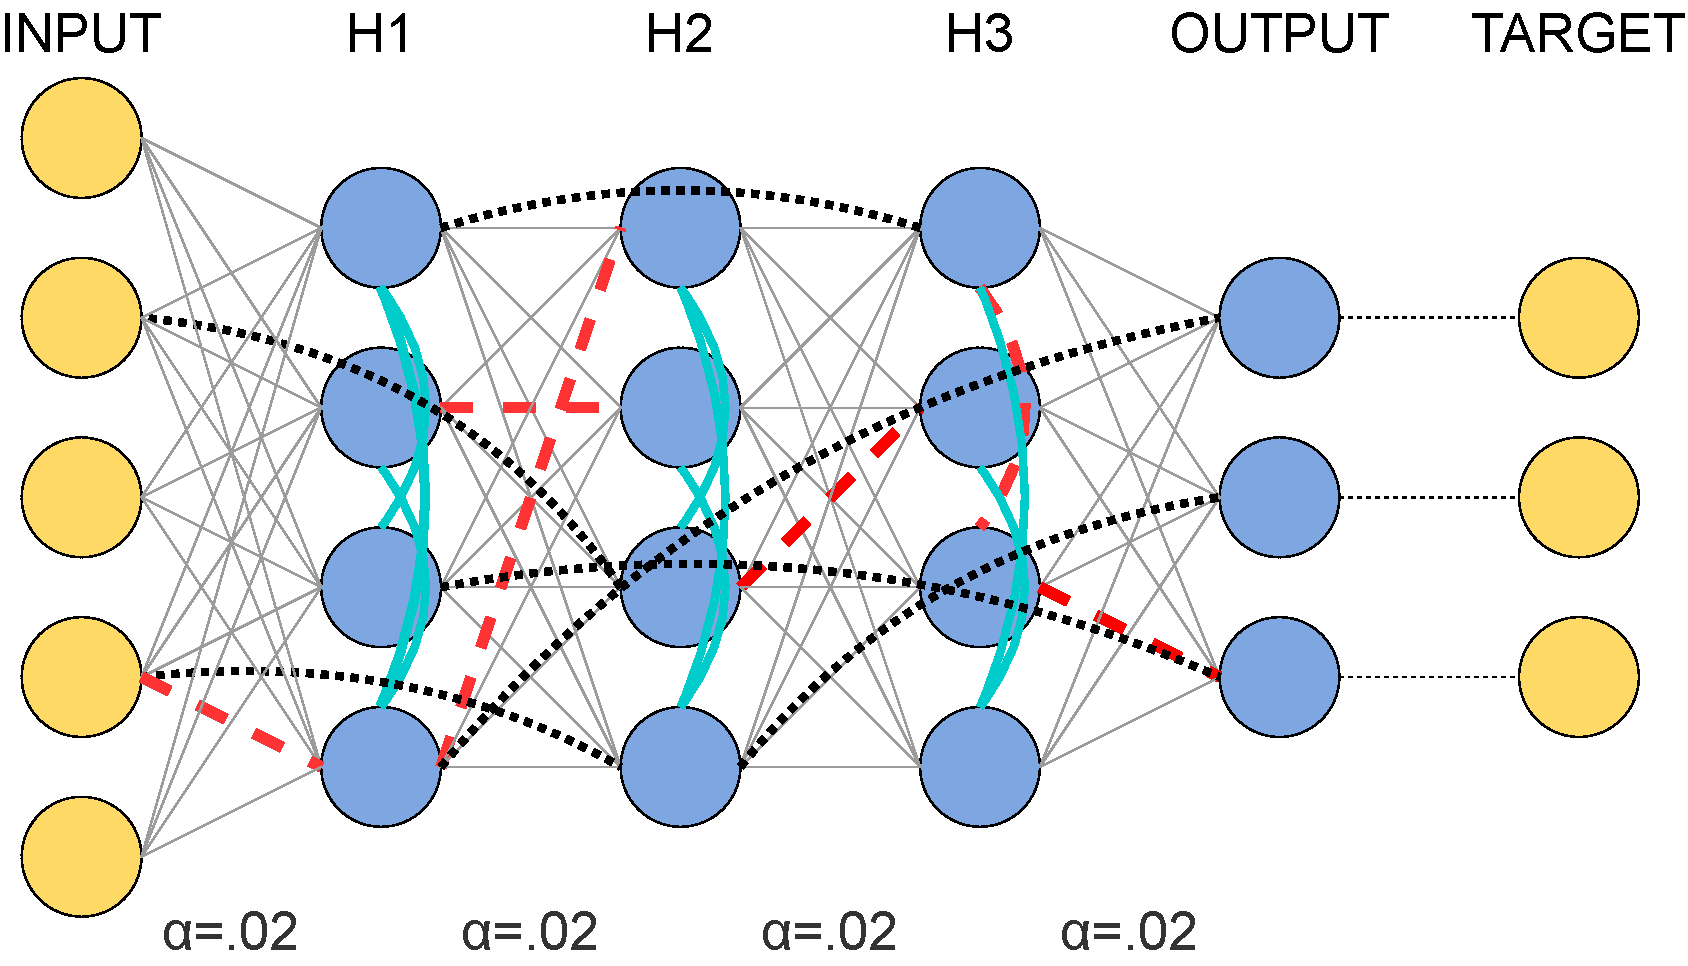
\includegraphics[width=\textwidth]{figures/topology_changes_step4.pdf}<4>
		\end{center}
	\end{textblock*}
	\begin{textblock*}{\textwidth}[.5, .5](.5\paperwidth, .825\paperheight)
		\begin{itemize}
			\item<1|only@1> Use original topology as starting point
			\item<1|only@1> Single global learning rate across all layers
		\end{itemize}
		\begin{itemize}
			\item<2|only@2> Make hidden layers fully-connected
		\end{itemize}
		\begin{itemize}
			\item<3|only@3> Consider each connection and remove with probability $p$
		\end{itemize}
		\begin{itemize}
			\item<4|only@4> For each removed connection, randomly connect two separated neurons
			\begin{itemize}
				\item<4|only@4> Only 1 connection per pair
				\item<4|only@4> No connections within input or output layers
			\end{itemize}
		\end{itemize}
	\end{textblock*}
\end{frame}

\section{Results}
\subsection{Performance comparison between topologies}
\begin{frame}
	\frametitle{Results: performance of network with layer-skipping connections}
	\begin{figure}
		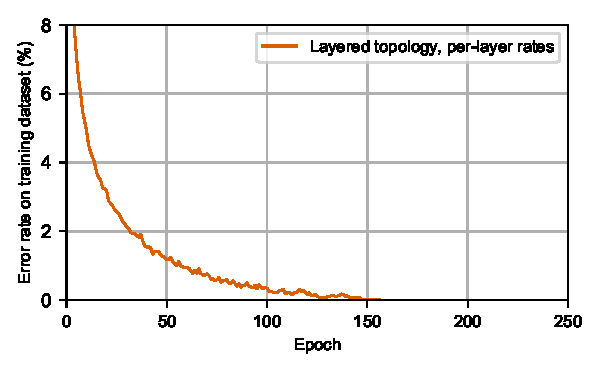
\includegraphics[width=\textwidth]{figures/performance_original.pdf}
	\end{figure}
\end{frame}
\begin{frame}
	\frametitle{Results: performance of network with layer-skipping connections}
	\begin{figure}
		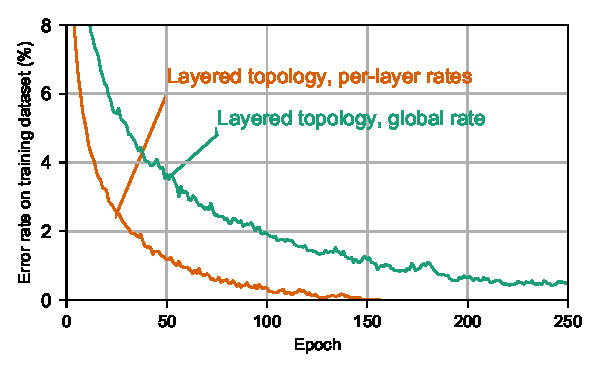
\includegraphics[width=\textwidth]{figures/performance_original+global.pdf}
	\end{figure}
\end{frame}
\begin{frame}
	\frametitle{Results: performance of network with layer-skipping connections}
	\begin{figure}
		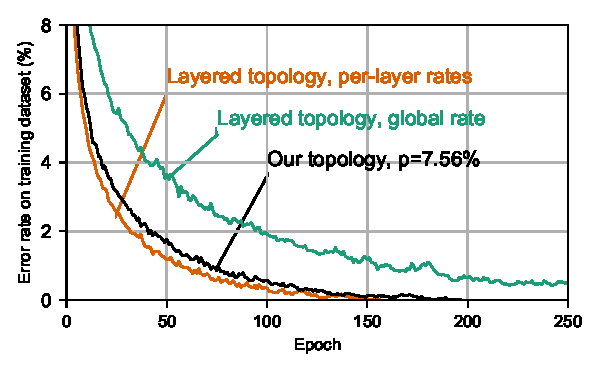
\includegraphics[width=\textwidth]{figures/performance_original+global+ours.pdf}
	\end{figure}
\end{frame}
\subsection{Layer training rate comparison between topologies}
\begin{frame}
	\frametitle{Results: effect on training rates of layers}
	\begin{figure}
		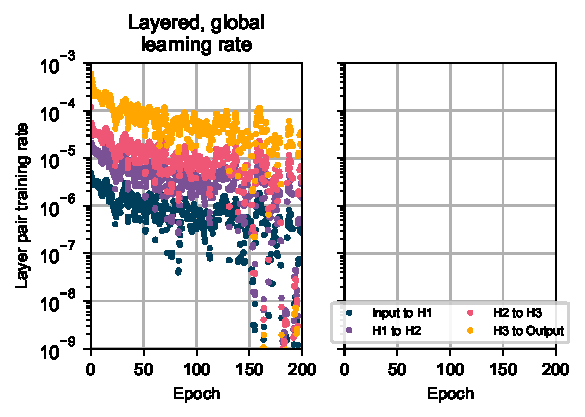
\includegraphics[width=\textwidth]{figures/perlayer_global.pdf}
	\end{figure}
\end{frame}
\begin{frame}
	\frametitle{Results: effect on training rates of layers}
	\begin{figure}
		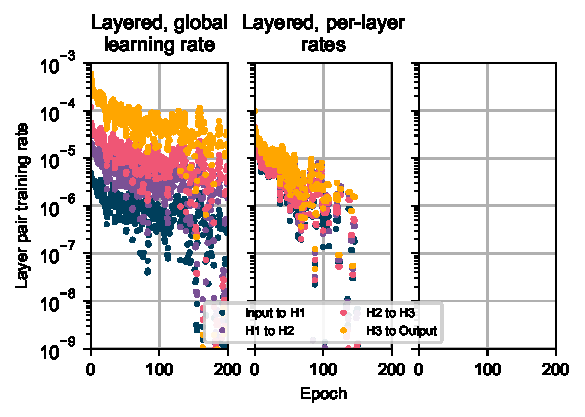
\includegraphics[width=\textwidth]{figures/perlayer_global+original.pdf}
	\end{figure}
\end{frame}
\begin{frame}
	\frametitle{Results: effect on training rates of layers}
	\begin{figure}
		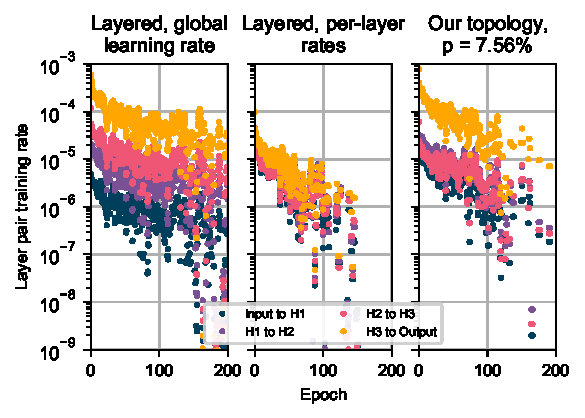
\includegraphics[width=\textwidth]{figures/perlayer_global+original+ours.pdf}
	\end{figure}
\end{frame}

\begin{frame}
	\frametitle{Results: takeaways}
\end{frame}

\section{Directions for future research}
\begin{frame}
	\frametitle{Directions for future research}
	\begin{itemize}
		\item<1-> Evaluate effectiveness on harder datasets, e.g. CIFAR, ImageNet, where network depth is very important
		\item<2-> Evaluate effect of $p$ on network test error
		\item<3-> Evaluate effectiveness on deeper networks
		\item<4-> Try training a network with added layer-skipping connections, then removing them afterwards
	\end{itemize}
\end{frame}

\begin{frame} % references slide

\end{frame}

\end{document}